\linenumbers
\footnotesize
\begin{verbatim}
#Date           Category        Amount  Margin   sub cat, automatic, date start, date end
forecast        Prêt            627.71  0.00   Prêt taux 1, PA, 15/01/2012
forecast        Prêt            151.61  10.00   Prêt taux 2, PA, 15/01/2012
forecast        Assurance       300.00  150.00              , PNA
forecast        Téléphonie      2.00    0.00   Free Mobile, PA, 10/01/2012, 10/01/2015, 2
forecast        Téléphonie      4.77    0.00   OVH,         PA, 01/01/2012
forecast        Cadeaux         5.00    0.00   MSF,                PA, 01/01/2012
forecast        Cadeaux         6.00    0.00   AIDES,              PA, 01/01/2012
forecast        Cadeaux         7.00    0.00   CARE,               PA, 01/01/2012
forecast        Cadeaux         6.00    0.00   ADECE,              PA, 01/01/2012
forecast        Cadeaux         10.00   0.00   Secours Catholique, PA, 01/01/2012
forecast        Administratif   218.06  0.00   Appel de fonds Syndic,          PA, 01/01/2012
forecast        Administratif   30.00   0.00   virement Epargne ,              PA, 01/01/2012
forecast        Administratif   2.40    0.00   Cotisation CNV Equipage Facile, PA, 01/01/2012
forecast        Administratif   5.40    0.00   Cotisation CNV Equipage 2,      PA, 01/01/2012
forecast        Administratif   3.62    0.00   Cotisation CNV Co-Equipage 2,   PA, 01/01/2012
forecast        Administratif   30.00   0.00   Assurance vie,                  PA, 01/01/2012
forecast        Administratif   500.00  150.00   , PNA
\end{verbatim}
\nolinenumbers
\normalsize

Le prévisionnel (\textit{forecast} en anglais) permet la décomposition en catégories contenant
chacune une ou plusieurs opérations. En Fig.~\ref{forecast:example} est donnée la structure
du prévisionel en exemple.

\begin{figure}
\centering
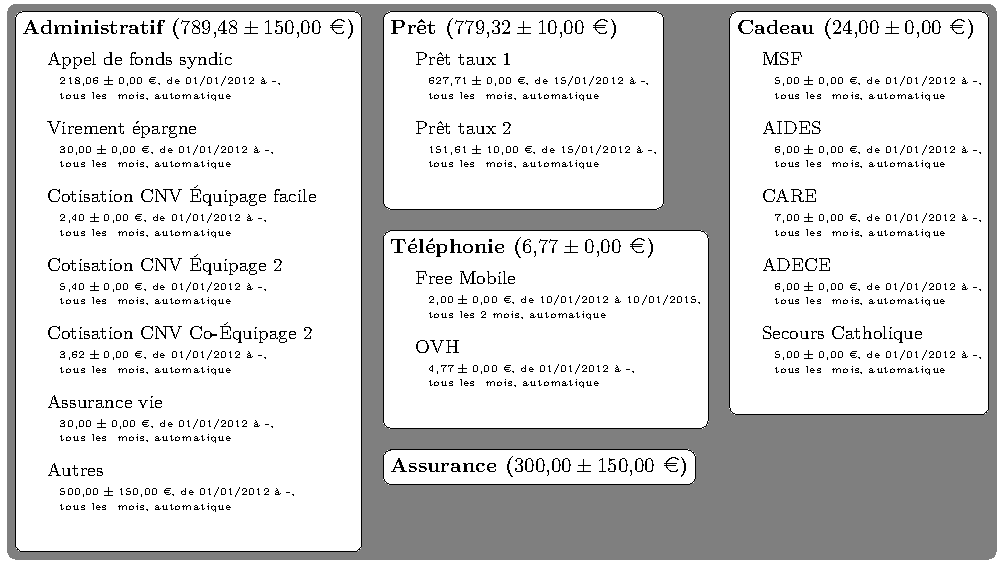
\includegraphics[width=\linewidth]{forecast_structure}
\caption{\label{forecast:example}Structure du prévisionnel de l'exemple.}
\end{figure}
